%! TEX root = main.tex

\graphicspath{{00_Images/13_chapter/}}

\chapter{Microphone Directivity and Models}

Microphones are classified according to the acoustic quantity they sense: the absolute pressure at a point, the spatial gradient of that pressure, or a weighted combination of both.
This distinction determines not only the directional response but also the sensitivity to source distance, and it underpins the design of every practical microphone pattern from the omnidirectional to the hypercardioid.

\section{Pressure Microphones}

A pressure microphone exposes only one face of its diaphragm to the sound field; the rear face is enclosed by a sealed cavity.
A narrow equalization vent connects the interior of that cavity to the ambient atmosphere, allowing slow static pressure changes to pass through without affecting the audio-band response, while remaining acoustically opaque to acoustic frequencies.
The incident plane wave \(\tilde{p} = \tilde{p}_0 e^{-jkx}\) acts directly on the exposed face, and the net driving force on a diaphragm of area \(S_D\) is simply
\[
\tilde{f}_D = \tilde{p} S_D
\]
Because the rear cavity is sealed, only the absolute pressure on the front face matters; the differential pressure across the diaphragm equals the incident pressure itself.

\begin{figure}[!htb]
    \centering
    \subfloat[Cross-section of a pressure-microphone capsule with equalization vent]{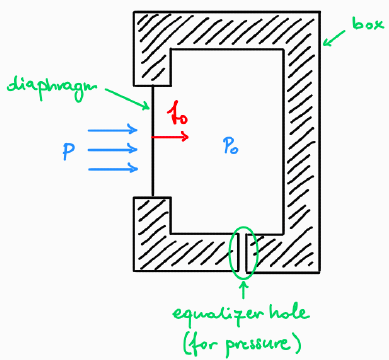
\includegraphics[height=0.2\textheight]{pressure_mic_structure.png}}
    \hfill
    \subfloat[Omnidirectionality condition: when \(\lambda \gg L\) the pressure is spatially uniform across the diaphragm]{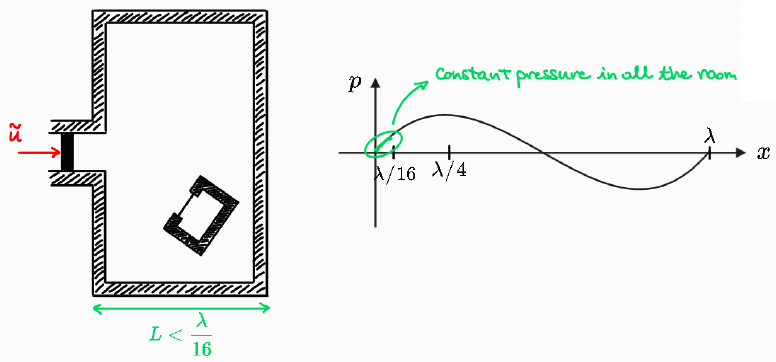
\includegraphics[height=0.2\textheight]{room.png}}
    \caption{Pressure microphone: capsule structure and the long-wavelength condition that guarantees omnidirectional response}
\end{figure}

As long as the acoustic wavelength \(\lambda\) is much larger than the microphone body (dimension \(L\)), the pressure does not vary appreciably from one side of the diaphragm to the other, and the output voltage is independent of the angle of incidence \(\theta\):
\[
v_P(\theta) = v_{P0}
\]
The pressure microphone is therefore inherently omnidirectional.
At high frequencies, where the microphone body becomes comparable to the wavelength, diffraction creates an acoustic shadow and the directional response departs from the circular polar pattern; this sets an upper frequency limit that scales inversely with capsule diameter, as discussed in the previous chapter on specifications.

\section{Pressure-Gradient Microphones}

A pressure-gradient microphone exposes both faces of the diaphragm directly to the sound field.
The diaphragm therefore responds to the pressure difference \(\tilde{p}_1 - \tilde{p}_2\) across its two sides, which is proportional to the local spatial derivative of the pressure field.
This differential coupling makes the transducer inherently directional.

\subsection{Force on the Diaphragm: Plane-Wave Excitation}

Let \(\tilde{p}_1\) and \(\tilde{p}_2\) denote the acoustic pressures at the front and rear faces of the diaphragm, separated along the acoustic axis by an effective path distance \(\Delta l\).
The net acoustic force on the diaphragm, projected onto its normal, is
\[
\tilde{f}_{D\perp} = (\tilde{p}_1 - \tilde{p}_2) S_D \cos\theta
\]
where \(\theta\) is the angle of incidence measured from the diaphragm axis, so that on-axis incidence corresponds to \(\theta = 0\).

\begin{figure}[!htb]
    \centering
    \subfloat[Differential pressure acting on the two faces of the diaphragm]{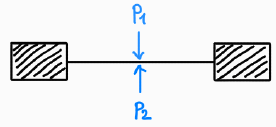
\includegraphics[height=0.18\textheight]{pressure_grad_mic_1.png}}
    \hfill
    \subfloat[Plane wave at angle \(\theta\) and the effective path difference \(\Delta l\) across the diaphragm]{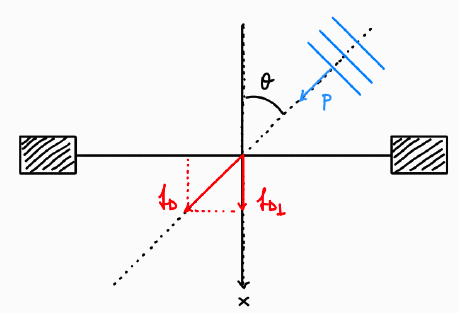
\includegraphics[height=0.18\textheight]{pressure_grad_mic_plane.png}}
    \caption{Pressure-gradient microphone: forces on the diaphragm faces and the geometry of oblique incidence}
\end{figure}

For small separations \(\Delta l\), the pressure difference is approximated to first order as
\[
\tilde{p}_1 - \tilde{p}_2 \approx -\frac{\partial \tilde{p}}{\partial x} \Delta l
\]
giving
\[
\tilde{f}_{D\perp} = -S_D \frac{\partial \tilde{p}}{\partial x} \Delta l \cos\theta
\]
The acoustic momentum equation (Newton's second law applied to a fluid element) relates the pressure gradient to the particle velocity:
\[
-\frac{\partial p}{\partial x} = \rho_0 \frac{\partial u}{\partial t}
\]
For harmonic excitation \(\tilde{u} = u_0 e^{j\omega t}\), the time derivative yields \(\partial\tilde{u}/\partial t = j\omega \tilde{u}\), so the normal force becomes
\[
\tilde{f}_{D\perp} = \rho_0 S_D \Delta l j\omega \tilde{u} \cos\theta = jk \rho_0 c \tilde{u} S_D \Delta l \cos\theta
\]
For a plane wave, \(\partial\tilde{p}/\partial x = -jk \tilde{p}\), which permits the force to be expressed directly in terms of pressure:
\[
\tilde{f}_{D\perp} = jk \tilde{p} S_D \Delta l \cos\theta, \qquad |\tilde{f}_{D\perp}| = \frac{\omega}{c} |\tilde{p}| S_D \Delta l |\cos\theta|
\]
The angular dependence \(|\cos\theta|\) implies that the response is maximum on-axis (\(\theta = 0^\circ\)), vanishes at \(\theta = \pm 90^\circ\), and reappears with opposite sign at \(\theta = 180^\circ\): the output voltage follows \(v_G(\theta) = v_{G0}\cos\theta\), which is the bidirectional or figure-eight polar pattern.

\begin{figure}[!htb]
    \centering
    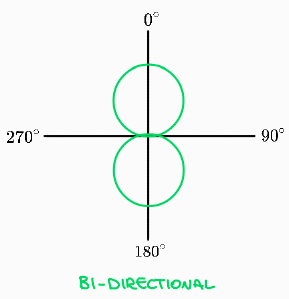
\includegraphics[width=0.38\textwidth]{bi_directional_pattern.png}
    \caption{Bidirectional (figure-eight) polar pattern of a pressure-gradient microphone for plane-wave excitation}
\end{figure}

\paragraph{Effective path difference} The value of \(\Delta l\) is set by the radiation impedance of the diaphragm rather than by its physical size alone.
For a rigid circular diaphragm of radius \(a\) acting as a piston in free space, the specific radiation impedance at low frequencies gives
\[
\Delta l_{\mathrm{rigid}} = \frac{4a}{3\pi} \approx \frac{a}{2}
\]
For a flexible disk vibrating in its first bending mode, the radiation impedance yields a somewhat larger effective path:
\[
\Delta l_{\mathrm{flex}} = \frac{\pi a}{4} \approx \frac{3a}{4}
\]
Both limiting cases confirm that \(\Delta l\) is of order \(a\), the diaphragm radius.

\subsection{Force on the Diaphragm: Spherical Waves and the Proximity Effect}

When the acoustic source is a point monopole at distance \(r\), the pressure field is spherical:
\[
\tilde{p}(r) = \tilde{A}_0 \frac{e^{-jkr}}{r}
\]
The radial pressure gradient is then
\[
\frac{\partial \tilde{p}}{\partial r} = -\frac{1+jkr}{r} \tilde{p}(r)
\]
and the normal diaphragm force becomes
\[
\tilde{f}_{D\perp} = \tilde{p}(r) \frac{1+jkr}{r} S_D \Delta l \cos\theta
\]
Taking the RMS magnitude and using the spherical-wave relation \(|\tilde{u}|_{\mathrm{rms}} = |\tilde{p}|_{\mathrm{rms}} \sqrt{1+(kr)^2} /(kr \rho_0 c)\):
\[
|\tilde{f}_{D\perp}|_{\mathrm{rms}} = |\tilde{p}|_{\mathrm{rms}} \frac{\sqrt{1+(kr)^2}}{r} \frac{\omega}{c} S_D \Delta l \cos\theta = |\tilde{u}|_{\mathrm{rms}} \omega \rho_0 S_D \Delta l \cos\theta
\]
It is convenient to define the distance factor
\[
\gamma = \frac{\sqrt{1+k^2r^2}}{r} = \frac{\sqrt{1+(r/r_0)^2}}{r}, \qquad r_0 = \frac{\lambda}{2\pi} \approx \frac{\lambda}{6}
\]
which quantifies how the effective pressure gradient scales with source distance at a given frequency.
Two asymptotic regimes emerge from this expression.
In the far field, where \(r \gg r_0\) (equivalently \(kr \gg 1\)), the factor \(\gamma \approx k\) and the gradient falls off as \(|\tilde{p}|/r\), consistent with ordinary spherical spreading.
In the near field, where \(r \ll r_0\) (equivalently \(kr \ll 1\)), the factor \(\gamma \approx 1/r\) and the gradient falls off as \(|\tilde{p}|/r^2\), an additional \(1/r\) roll-off relative to the pressure itself.
The crossover distance \(r_0 = \lambda/(2\pi)\) increases with decreasing frequency.
At a fixed source-to-microphone distance \(r\), low frequencies satisfy \(r \ll r_0\) and therefore lie in the near-field regime, while high frequencies satisfy \(r \gg r_0\) and follow the far-field law.
Consequently, at close distances a directional microphone receives a relative boost of low frequencies compared to high frequencies, since the near-field enhancement of the gradient is more pronounced at low frequencies: this is the proximity effect.
The effect grows stronger as the source approaches the microphone and disappears at large distances, where all frequencies are in the far field.
Most directional microphones incorporate a high-pass filter in their equalization to compensate for this bass enhancement in close-range use.

\begin{figure}[!htb]
    \centering
    \subfloat[Output voltage as a function of frequency for several source distances]{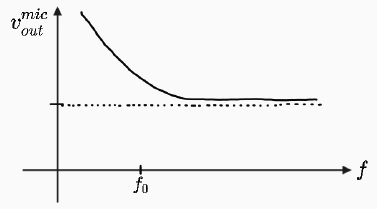
\includegraphics[width=0.46\textwidth]{v_mic_out.png}}
    \hfill
    \subfloat[Normal diaphragm force \(|\tilde{f}_{D\perp}|\) versus distance, showing the transition between \(1/r^2\) near-field and \(1/r\) far-field scaling]{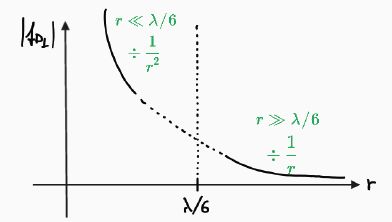
\includegraphics[width=0.46\textwidth]{f_D_perp.png}}
    \caption{Distance and frequency dependence of the pressure-gradient microphone response, illustrating the physical origin of the proximity effect}
\end{figure}

\section{Combination Microphones}

Adding the output of a pressure element to that of a pressure-gradient element produces a directional pattern intermediate between the omnidirectional and the bidirectional extremes.
Denoting the individual outputs as \(v_P(\theta) = v_{P0}\) and \(v_G(\theta) = v_{G0}\cos\theta\), the total microphone voltage is
\[
v_M(\theta) = v_{P0} + v_{G0}\cos\theta = v_{P0}\left(1 + B\cos\theta\right), \qquad B = \frac{v_{G0}}{v_{P0}}
\]
The on-axis value \(v_M(0) = v_{P0}(1+B)\) is the maximum output, so the response normalized to its on-axis maximum defines the directivity function
\[
D(\theta) = \frac{v_M(\theta)}{v_M(0)} = \frac{1+B\cos\theta}{1+B}, \qquad -1 \leq D(\theta) \leq 1
\]
The polar pattern in decibels is obtained as \(20\log_{10}|D(\theta)|\).

\begin{figure}[!htb]
    \centering
    \subfloat[Schematic superposition of pressure and gradient outputs]{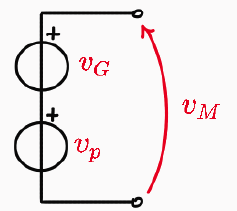
\includegraphics[height=0.2\textheight]{mic_combination.png}}
    \hspace{1cm}
    \subfloat[Cardioid polar pattern (\(B = 1\)): null at \(\theta = 180^\circ\), maximum at \(\theta = 0^\circ\)]{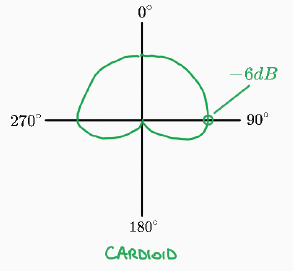
\includegraphics[height=0.2\textheight]{cardioid_pattern.png}}
    \caption{Combination microphone: superposition of pressure and gradient components, with the cardioid (\(B = 1\)) as the most common special case}
\end{figure}

The three canonical limiting patterns correspond to \(B = 0\) (only the pressure component survives, \(D = 1\), omnidirectional), \(B = 1\) (cardioid, \(v_M = v_{P0}(1 + \cos\theta)\), zero at \(\theta = 180^\circ\)), and \(B \to \infty\) (only the gradient survives, \(D \to \cos\theta\), bidirectional figure-eight).
The cardioid case at \(B = 1\) is worth noting in detail: the output at \(\theta = 0^\circ\) equals \(2v_{P0}\), at \(\theta = 90^\circ\) it equals \(v_{P0}\), and at \(\theta = 180^\circ\) it is exactly zero.

\begin{figure}[!htb]
    \centering
    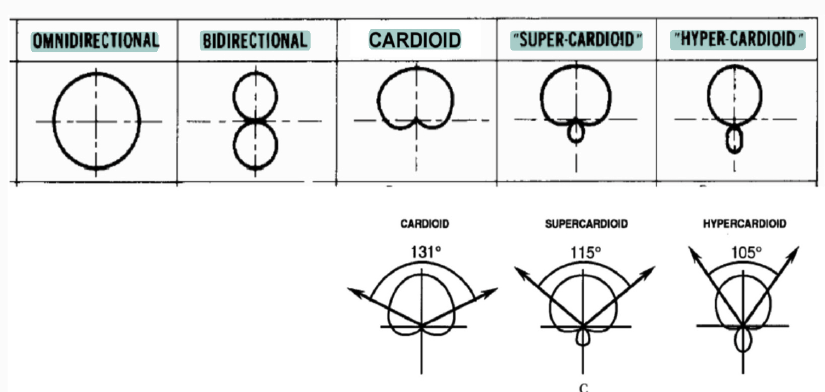
\includegraphics[width=0.65\textwidth]{directivity_pattern.png}
    \caption{A family of polar patterns generated by the combination formula for representative values of \(B\): omnidirectional, cardioid, supercardioid, hypercardioid, and bidirectional}
\end{figure}

\section{Directivity Factor and Polar Patterns}

\subsection{Definition of the Directivity Factor}

A quantitative comparison of directional microphones requires a single figure of merit that captures how much a pattern favors the on-axis direction over a diffuse field.
The directivity factor \(Q\) is defined in a homogeneous, isotropic sound field, where the RMS pressure \(p_{\mathrm{rms}}\) is the same from every direction.
The infinitesimal mean acoustic power arriving from a solid-angle element \(dA = r^2\sin\theta d\theta d\phi\) is
\[
d\overline{W}_A = \frac{p_{\mathrm{rms}}^2}{\rho_0 c} r^2\sin\theta d\theta d\phi
\]
since the ratio \(\mathrm{Re}[Z_S]/|Z_S|^2 = 1/(\rho_0 c)\) for a spherical wave in the far field.

\begin{figure}[!htb]
    \centering
    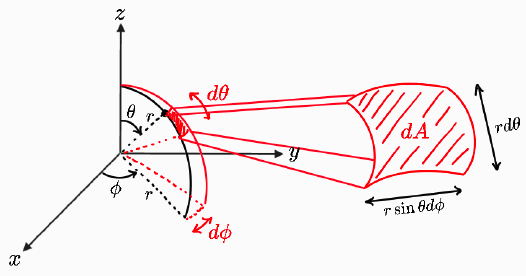
\includegraphics[width=0.50\textwidth]{polar_coord.png}
    \caption{Spherical coordinate geometry for the integration of acoustic power over all incident directions}
\end{figure}

A microphone with directivity function \(D(\theta)\) weights the received power by \(D^2(\theta)\):
\[
d\overline{W}_{A,M} = \frac{p_{\mathrm{rms}}^2}{\rho_0 c} D^2(\theta) r^2\sin\theta d\theta d\phi
\]
Integrating over the full sphere and exploiting azimuthal symmetry:
\[
\overline{W}_{A,M} = \frac{2\pi r^2 p_{\mathrm{rms}}^2}{\rho_0 c}\int_0^{\pi} D^2(\theta)\sin\theta d\theta
\]
For the omnidirectional reference, \(D = 1\) and \(\int_0^\pi\sin\theta d\theta = 2\), so \(\overline{W}_{A,\mathrm{omni}} = 4\pi r^2 p_{\mathrm{rms}}^2/(\rho_0 c)\).
The directivity factor is accordingly defined as
\[
Q = \frac{\overline{W}_{A,\mathrm{omni}}}{\overline{W}_{A,M}} = \frac{2}{\displaystyle\int_0^{\pi} D^2(\theta)\sin\theta d\theta} \geq 1
\]
A directional microphone, by excluding power arriving from unfavorable directions, receives less total power than an omnidirectional one in the same diffuse field, hence \(Q \geq 1\).

\subsection{Directivity Factor for the General Pattern}

Substituting \(D(\theta) = (1+B\cos\theta)/(1+B)\) and evaluating the key integral:
\[
\int_0^{\pi}(1+B\cos\theta)^2\sin\theta d\theta = \frac{6+2B^2}{3}
\]
the directivity factor takes the closed form
\begin{equation}
Q(B) = \frac{3(1+B)^2}{3+B^2}.
\label{eq:directivityFactor}
\end{equation}
The derivative with respect to \(B\) is
\[
\frac{\partial Q}{\partial B} = \frac{6(1+B)(3-B)}{(3+B^2)^2}
\]
which vanishes at \(B = 3\), confirming a maximum at that point with value \(Q_{\mathrm{max}} = Q(3) = 4\), realized by the hypercardioid pattern.

\begin{figure}[!htb]
    \centering
    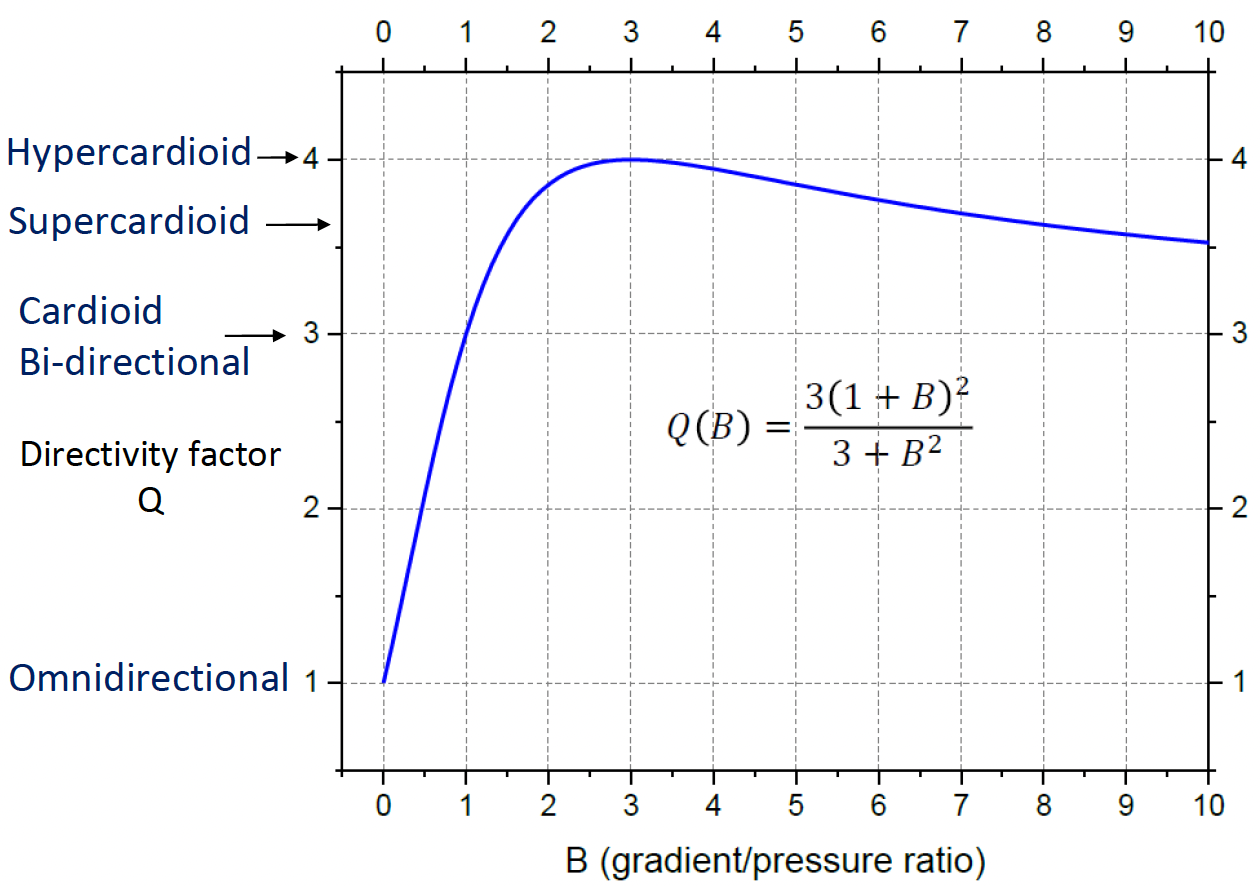
\includegraphics[width=0.55\textwidth]{Q_Factor_Mic.png}
    \caption{Directivity factor \(Q\) as a function of the mixing ratio \(B\), reaching its maximum \(Q = 4\) at \(B = 3\) (hypercardioid)}
\end{figure}

\subsection{Front-to-Rear Ratio}

The front-to-rear ratio \(FR\) quantifies how effectively the microphone rejects sound arriving from the rear hemisphere:
\[
FR = \frac{\overline{W}_{A,\mathrm{front}}}{\overline{W}_{A,\mathrm{rear}}} = \frac{\displaystyle\int_0^{\pi/2} D^2(\theta)\sin\theta d\theta}{\displaystyle\int_{\pi/2}^{\pi} D^2(\theta)\sin\theta d\theta}
\]
Evaluating with the general directivity function gives
\[
FR(B) = \frac{3+3B+B^2}{3-3B+B^2}
\]
Differentiating:
\[
\frac{\partial FR}{\partial B} = \frac{6(3-B^2)}{(3-3B+B^2)^2}
\]
which is zero at \(B = \sqrt{3}\): the front-to-rear ratio is maximized by the supercardioid pattern (\(B = \sqrt{3} \approx 1.7\)).
Note that the hypercardioid (\(B = 3\)) and the supercardioid (\(B = \sqrt{3}\)) optimize two different objectives, and no single value of \(B\) simultaneously maximizes both \(Q\) and \(FR\).

\begin{figure}[!htb]
    \centering
    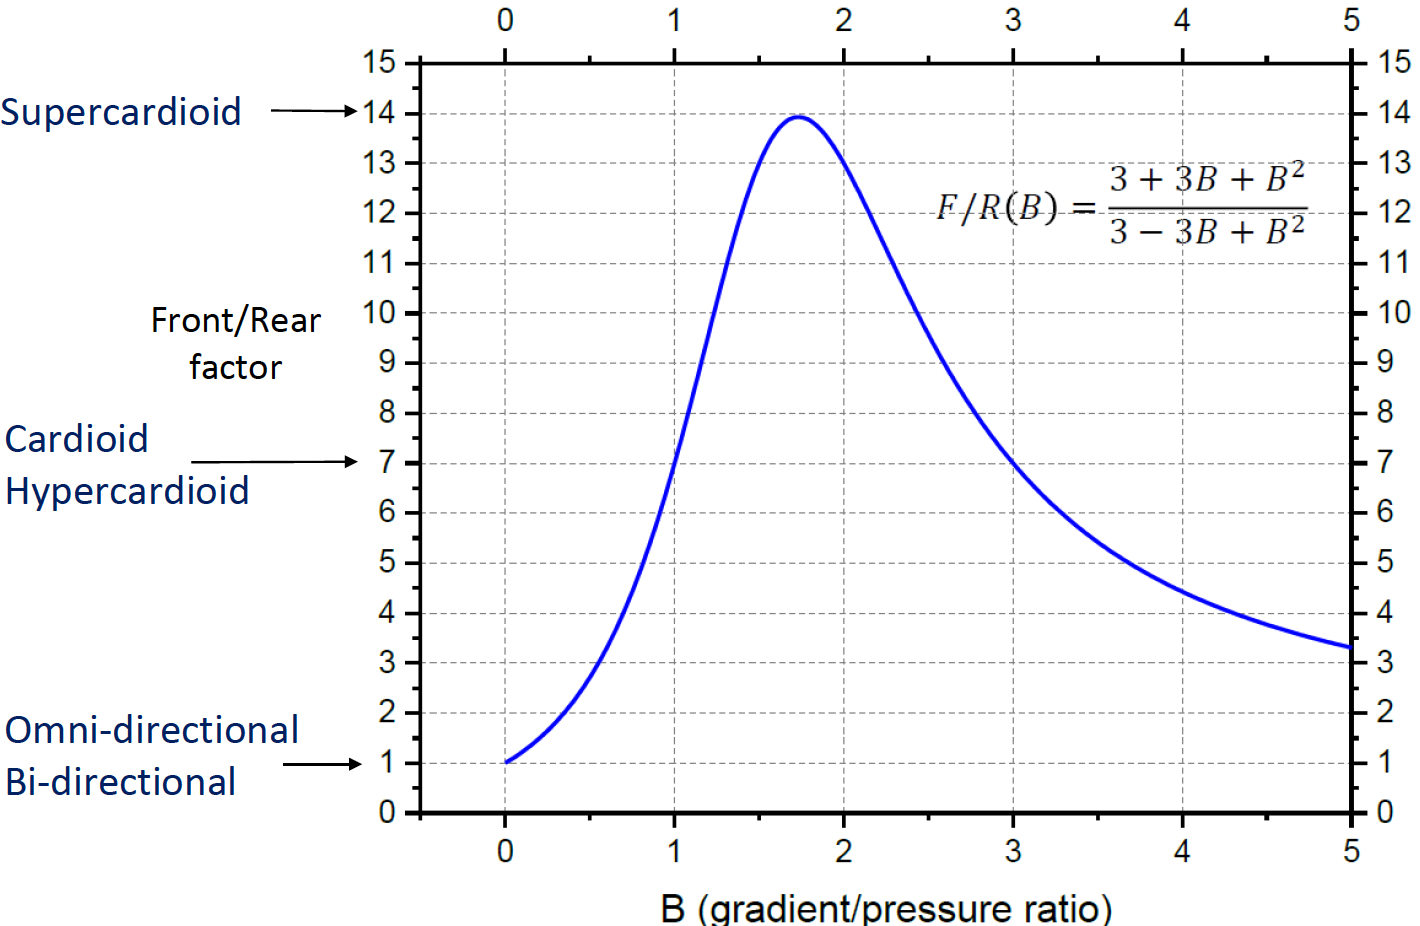
\includegraphics[width=0.55\textwidth]{Front_Rear_Ratio.png}
    \caption{Front-to-rear ratio \(FR\) as a function of \(B\), reaching its maximum at \(B = \sqrt{3}\) for the supercardioid}
\end{figure}

\subsection{Summary of Polar Patterns}

The five standard polar patterns, their mixing ratios, directivity factors from equation \eqref{eq:directivityFactor}, and front-to-rear ratios are collected in table \ref{tab:polarPatterns}.

\begin{table}[!htb]
\centering
\renewcommand{\arraystretch}{1.3}
\begin{tabular}{cccc}
\hline
\textbf{Pattern} & \textbf{\(B = v_{G0}/v_{P0}\)} & \textbf{Directivity factor \(Q\)} & \textbf{Front-to-rear \(FR\)} \\
\hline
Omnidirectional & \(0\)         & \(1\)        & \(1\)  \\
Bidirectional   & \(\infty\)    & \(3\)        & \(1\)  \\
Cardioid        & \(1\)         & \(3\)        & \(7\)  \\
Hypercardioid   & \(3\)         & \(4\)        & \(7\)  \\
Supercardioid   & \(\sqrt{3}\)  & \(\approx 3.7\) & \(14\) \\
\hline
\end{tabular}
\caption{Standard polar patterns and their directivity metrics}
\label{tab:polarPatterns}
\end{table}

Several observations are noteworthy.
The bidirectional and cardioid patterns share \(Q = 3\), despite their different spatial geometry: the bidirectional achieves this through figure-eight nulls at \(\pm 90^\circ\), while the cardioid achieves the same directivity through its smooth rear null at \(180^\circ\).
The hypercardioid at \(B = 3\) achieves the maximum directivity \(Q = 4\), meaning it captures only one quarter of the power received by an omnidirectional microphone in the same diffuse field; however, its front-to-rear ratio of \(7\) is identical to that of the cardioid, because the hypercardioid has a small but non-zero rear lobe.
The supercardioid at \(B = \sqrt{3}\) maximizes the front-to-rear ratio to \(14\), providing the strongest rear rejection at the cost of slightly reduced \(Q\); it is the preferred pattern when ambient noise arrives predominantly from behind the performer.

\section{Physical Realization: Rear-Cavity Model}

The combination formula \(v_M = v_{M0}(1 + B\cos\theta)\) is not merely an abstract superposition of two idealized transducers but can be realized acoustically within a single capsule by introducing a controlled path to the rear of the diaphragm.

\subsection{Structure and Circuit Model}

In the combined microphone, the rear face of the diaphragm communicates with the outside through a back cavity containing an acoustic compliance \(C_A\) (the enclosed air volume) and an acoustic resistance \(R_A\) (a resistive screen or narrow slot).
The front face is exposed directly to the incident field at position \(x_1\), while the rear opening samples the field at a displaced position.

\begin{figure}[!htb]
    \centering
    \subfloat[Physical model of the rear cavity]{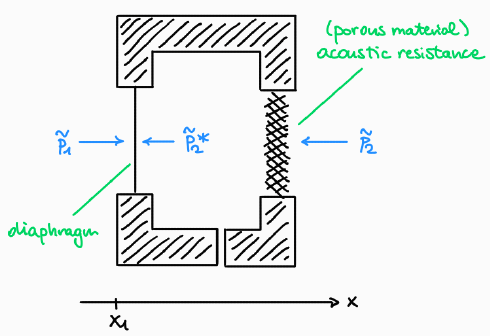
\includegraphics[height=0.21\textheight]{pressure_plus_gradient_mic_model.png}}
    \hfill
    \subfloat[Equivalent acoustic circuit with compliance \(C_A\), resistance \(R_A\), and diaphragm impedance \(Z_{AD}\)]{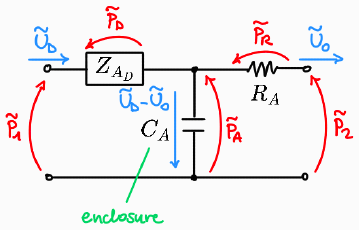
\includegraphics[height=0.21\textheight]{pressure_plus_grad_mic_circuit.png}}
    \caption{Combined pressure and pressure-gradient microphone: rear-cavity structure and its equivalent acoustic circuit}
\end{figure}

For a plane wave \(\tilde{p} = p_0 e^{-jkx}\), the front pressure is \(\tilde{p}_1 = p_0 e^{-jkx_1}\) and the pressure at the rear opening is, to first order in \(\Delta l\),
\[
\tilde{p}_2 = \tilde{p}_1\left(1 - j\frac{\omega}{c} \Delta l \cos\theta\right)
\]
Applying acoustic Kirchhoff laws to the equivalent circuit, with \(\tilde{U}_D\) and \(\tilde{U}_0\) denoting the volume velocities at the diaphragm and the rear port respectively, gives the pair of equations:
\[
\begin{cases}
\tilde{p}_1 = \dfrac{1}{j\omega C_A}(\tilde{U}_D - \tilde{U}_0) + Z_{AD} \tilde{U}_D \\[6pt]
\tilde{p}_2 = \dfrac{1}{j\omega C_A}(\tilde{U}_D - \tilde{U}_0) - R_A \tilde{U}_0
\end{cases}
\]
where \(Z_{AD}\) is the radiation impedance of the diaphragm.

\subsection{Differential Pressure and the Mixing Parameter}

Solving for the differential pressure \(\tilde{p}_D\) acting across the diaphragm:
\[
\tilde{p}_D = \tilde{p}_1\;\frac{Z_{AD} R_A\!\left[1 + \dfrac{\Delta l\cos\theta}{c R_A C_A}\right]}{Z_{AD} R_A - j \dfrac{R_A + Z_{AD}}{\omega C_A}}
\]
Defining the frequency-dependent complex amplitude
\[
A = \frac{Z_{AD} R_A}{Z_{AD} R_A - j \dfrac{R_A + Z_{AD}}{\omega C_A}}
\]
and the dimensionless mixing parameter
\[
B = \frac{\Delta l}{c R_A C_A}
\]
the magnitude of the net diaphragm force is
\[
|\tilde{f}_D| = \tilde{p}_D S_D = \tilde{p}_1 S_D |A| (1 + B\cos\theta)
\]
The output voltage, proportional to this force, recovers the general combination pattern:
\[
\tilde{v}_M = \tilde{v}_{M0} (1 + B\cos\theta)
\]
The mixing ratio \(B\) is governed by the acoustic time constant \(R_A C_A\) of the rear cavity: a shorter time constant (smaller compliance or larger resistance) increases \(B\), shifting the pattern from omnidirectional toward the hypercardioid.
At \(B = 0\), corresponding to a sealed cavity (\(R_A \to \infty\)), only the pressure component survives and the pattern is omnidirectional.
As \(B\) increases through \(1\), \(\sqrt{3}\), and \(3\), the capsule realizes the cardioid, supercardioid, and hypercardioid patterns in turn.
Multiple polar patterns can therefore be selected from a single capsule by varying the acoustic resistance of the rear cavity, a principle exploited in multi-pattern studio microphones.
